\chapter{Definite Assignment}
\label{c_definite_assignment}

The Whiley programming language requires that variables are known at \gls{compile_time} to be {\em definitely assigned} (i.e. that they are defined before used).  A conservative approach is taken to determining whether or not this is the case.  This ensures the language can be compiled efficiently, but also means that some provably safe programs are not valid Whiley programs.  In this chapter, we specify the process by which definite assignment is determined.

\section{Overview}

The following illustrates a simple function which will be rejected by the compiler because it cannot determine definite assignment for all variables.  The function is said to {\em fail definite assignment}:

\begin{lstlisting}
function f(int x) -> (int r):
   int y
   //
   if x < 0:
       y = 1
   //
   return x + y
\end{lstlisting}

In the above program, variable \lstinline{y} is {\em not} definitely assigned before its use in the \lstinline{return} statement.  This is because there is an \gls{execution_path} through the function which reaches the \lstinline{return} statement and on which variable \lstinline{y} is not defined (see Figure~\ref{f:c8_cfg_1}).  In fact, there are {\em two} possible execution paths through this function, but variable \lstinline{y} is only defined on one of them.  Observe that, since it is a parameter, variable \lstinline{x} is automatically considered to have been defined on entry to the function.


\begin{figure}[!t]
\centering
  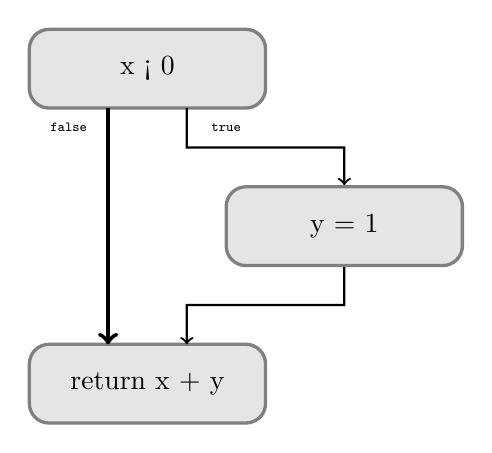
\begin{tikzpicture}[
    graynode/.style={
      rectangle, 
      draw=gray!100, 
      fill=gray!20.5, 
      very thick, 
      minimum size=5mm,
      minimum height=1cm,
      minimum width=3cm,
      rounded corners=0.25cm
    }
    ]
    \node[graynode] (l1) at (0,4cm) {\lstinline{x < 0}};
    \node at (1,3.25) {\tiny${\tt true}$};
    \node at (-1,3.25) {\tiny${\tt false}$};
    \node[graynode] (l2) at (2.5cm,2cm) {\lstinline{y = 1}};
    \node[graynode] (l3) at (0,0) {\lstinline{return x + y}};
    \draw[thick,->] (l1)++(0.5,-0.5) -- (0.5,3) -- (2.5,3) -- (l2);
    \draw[thick,->] (l2) -- (2.5,1) -- (0.5,1) -- (0.5,0.5);
    \draw[ultra thick,->] (-0.5,3.5) -- (-0.5,0.5);
  \end{tikzpicture}
\caption{Control-Flow Graph for function \lstinline{f()}.  On the bold path, \lstinline{y} is undefined.}
\label{f:c8_cfg_1}
\end{figure}

\subsection{Loops}

The treatment of loops with respect to definite assignment warrants special attention.  Recall the mechanism for determining definite assignment is conservative.  In the context of loops, it simply assumes {\em every loop can be executed zero or more times} (i.e. even if this is not correct).  The following illustrates:

\begin{lstlisting}
function f(int x) -> int:
   int y
   //
   while x < 0:
       y = 1
       x = x + 1
   //
   return x + y
\end{lstlisting}

The above function fails definite assignment because variable \lstinline{y} is not defined when zero iterations of the loop are executed (e.g. when \lstinline{x==0} on entry).  To illustrate the conservative nature of definite assignment, consider this variation:

\begin{lstlisting}
function ten() -> int:
   int x = 0
   int y
   //
   while x < 10:
       y = 1
       x = x + 1
   //
   return y
\end{lstlisting}

Here, it can be shown that \lstinline{y==1} must hold when the \lstinline{return} statement is reached.  Nevertheless, this function fails definite assignment because of the assumption that the loop executes {\em zero} or more iterations.

\subsection{Infeasible Paths}

Functions and methods may contain \glslink{infeasible_path}{infeasible paths} which are valid execution paths that, in practice, cannot be executed.  The mechanism for checking definite assignment assumes for simplicity that any valid path can be executed.  This means that some programs will fail definite assignment, even though they can be shown as safe.   The following illustrates such a program:

\begin{lstlisting}
function abs(int x) -> int:
    int y
    //
    if x >= 0:
        y = x
    //
    if x < 0:
        y = -x
    //
    return y
\end{lstlisting}

This function contains four valid execution paths which can be denoted by \lstinline{ff}, \lstinline{tf}, \lstinline{ft}, \lstinline{tt} where, for example, \lstinline{tf} represents the path where the first condition evaluates to \lstinline{true} and the second to \lstinline{false}.  However, it is easy to see that execution paths \lstinline{ff} and \lstinline{tt} are infeasible.  Furthermore, that on the other two paths, \lstinline{tf} and \lstinline{ft}, variable \lstinline{y} is definitely assigned at the \lstinline{return} statement.  Despite this, the above function fails definite assignment because the mechanism considers all valid paths whilst ignoring infeasible execution paths.

\subsection{Partial Assignments}

A variable will never be considered definitely assigned after the application of one or more {\em partial assignments}.  The following illustrates a program which fails definite assignment even though it can be shown as safe:

\begin{lstlisting}
type Point is {int x, int y}

function Point(int x, int y) -> Point:
    Point p
    p.x = x
    p.y = y
    return p
\end{lstlisting}

In the above program, the variable \lstinline{p} can be shown as definitely assigned at the \lstinline{return} statement.  Nevertheless, the conservative mechanism for checking definite assignment will reject this program because variable \lstinline{p} is initialised via partial assignments.  

\section{Description}

Definite assignment is defined over the \gls{control_flow_graph} of a code block, such as a \lstinline{requires} or \lstinline{ensures} clause, or the body of a function or method.  Appendix~\S\ref{c_cfg} details the process for constructing a control-flow graph from a block of code.  

Definite assignment considers the set of all {\em valid paths} in a \gls{control_flow_graph}.  A valid path is a path through the graph starting from its root.  Every vertex in the graph is associated with a set of variables which are {\em defined} at that vertex, as well as those which are {\em used} at that vertex.  A variable $x$ is said to be {\em definitely assigned} on entry to a vertex $v$ if, for every valid path which includes $v$, some ancestor vertex $u$ exists on which $x$ is defined.

\subsection{Definitions and Uses}

A \gls{variable_definition} occurs at a vertex $v$ which contains a direct assignment (recall~\S\ref{c_stmt_assign}), or an initialisation of (recall~\S\ref{c_stmts_var_decl}), one or more variables.  Assignments to fields, array elements or dereferenced references are not direct and do not define variables.  A vertex may define multiple variables if it corresponds to a multiple assignment which directly assigns those variables.  Finally, the parameters of a function, method or invariant block are treated as being defined on entry. 

A \gls{variable_use} occurs at a vertex $v$ which directly refers to that variable in some expression other than an \lstinline{LVal}.  However, referring to a variable indirectly through a dereference expression does not constitute a variable use.
